%% Chapter 15: Parameterized Algorithms I
%% Status: drafted; figures are still placeholders.
%%
%% Written against "material/slides/aa-fpt.pdf" (Hans Bodlaender), slides 1-66:
%% definitions, four branching algorithms, kernelisation, and the first two
%% kernels.  Slides 67-83 (Nemhauser-Trotter and the cluster editing kernel)
%% belong to chapter 17.
%%
%% The pool items on Directed k-Path and one-sided error are answered in
%% chapter 18; no deck in material/ covers them yet.

\chapter{Parameterized Algorithms I}
\label{ch:fpt-i}

Parameterized complexity refuses to measure the difficulty of an instance by its
length alone. Real instances are rarely arbitrary: the graph may be enormous but
the solution we are looking for small, the data may be huge but the number of
errors in it few. So we isolate a second number $k$ --- the size of the
solution, the number of allowed edits, the treewidth --- and ask for algorithms
whose exponential behaviour is confined to $k$, with only a polynomial in the
input size beside it. Astonishingly often, this works.

\begin{goals}
  \poolgoal{define a parameterized problem, FPT, XP and para-NP-hard}
  \poolgoal{describe the idea of a branching algorithm in general}
  \poolgoal{define \lang{Vertex Cover} and show that it can be solved in FPT
        time using a branching algorithm}
  \poolgoal{define \lang{Cluster Editing} and give a branching algorithm for it}
  \poolgoal{give one parameterized problem that is para-NP-complete}
  \poolgoal{define the notion of a kernel}
  \poolgoal{show that a problem is FPT if and only if it has a kernel}
  \poolgoal{show that \lang{Vertex Cover} has a kernel of size $\bigoh{k^2}$}
  \poolgoal{define \lang{Convex String Recoloring} and show that it has a kernel
        of size $\bigoh{k^2}$}
  \goalitem{give the branching algorithms for \lang{Independent Set} on planar
        graphs and for \lang{Closest String}, and analyse them}
\end{goals}

%==============================================================================
\section{Parameters}
\label{sec:fpt-parameters}
%==============================================================================

Consider the question: \emph{can seven vertices be chosen so that every edge has
one of them?} On a graph with a million vertices this is a question about a
million-vertex object, and the trivial algorithm --- try every set of seven ---
takes $\binom{10^6}{7} \approx 10^{38}$ steps. But seven is a small number, and
it is reasonable to hope that the algorithm should be exponential in seven
rather than in a million.

That hope is the whole subject. We attach to every instance a second number,
called the \emph{parameter}, and ask for a running time that is polynomial in
the input size with all the exponential behaviour pushed into a function of the
parameter alone.

\begin{definition}[Parameterized problem]\label{def:fpt-problem}
A \emph{parameterized problem} is a subset of $\{0,1\}^{*} \times \N$. An
instance is a pair $(x,k)$, where $x$ is the input in the usual sense and $k$ is
the \emph{parameter}.
\end{definition}

For a graph problem the usual choice is the size of the solution asked for, and
this is called the \emph{standard parameterization}: given a graph $G$ and an
integer $k$, with $k$ as the parameter, does $G$ have a $\ldots$ of size at
least (or at most) $k$? Three examples show at once that the parameter does not
by itself make anything easy.

\begin{example}[Three parameterized problems]\label{ex:fpt-three}
\lang{Graph Coloring} asks whether $G$ has a proper colouring with $k$ colours.
This is \textrm{NP}-complete already for $k = 3$, so a small parameter is no
help at all.

\lang{Clique} asks whether $G$ has a clique of size at least $k$. It is solvable
in $\bigoh{n^{k+1}}$ time by trying every $k$-set --- polynomial for each fixed
$k$, but with $k$ in the exponent, so useless for $k = 20$ on a large graph.
A more complicated algorithm, due to \citet{NesetrilPoljak1985}, uses fast
matrix multiplication to bring this down to $\bigoh{n^{\omega k/3}}$, where
$\omega < 2.373$ is the exponent of \cref{ch:exact-i} --- about $n^{0.79k}$ ---
and the exponent still grows with $k$.

\lang{Vertex Cover} asks whether $G$ has a vertex cover of size at most $k$. It
is solvable in $\bigoh{2^k(n+m)}$ time, and that is a different shape of running
time entirely: for $k = 20$ and a graph of a million edges it is a few hundred
million steps, which is a second's work.
\end{example}

\begin{intuition}
The three examples are the three possibilities, and telling them apart is what
the theory is for. $\bigoh{2^k \cdot n}$ and $\bigoh{n^k}$ look similar written
on a slide and are nothing alike in practice: in the first the parameter and the
input size are separated, in the second they are multiplied together in the
exponent. The point of parameterized complexity is to make that difference a
formal one, so that it can be proved rather than observed.
\end{intuition}

%==============================================================================
\section{The classes}
\label{sec:fpt-classes}
%==============================================================================

The definition that separates \lang{Vertex Cover} from \lang{Clique} in
\cref{ex:fpt-three} is the following, proposed by Downey and Fellows.

\begin{definition}[FPT]\label{def:fpt}
A parameterized problem is \emph{fixed parameter tractable}, written
$\mathrm{FPT}$, if it has an algorithm deciding instances $(x,k)$ in time
\[ f(k) \cdot p(|x|) \]
for some computable function $f$ and some polynomial $p$.
\end{definition}

The function $f$ is unrestricted: it may be $2^k$, or $k!$, or a tower of
exponentials. What matters is that it does not touch $|x|$.

\begin{definition}[XP]\label{def:xp}
A parameterized problem is in $\mathrm{XP}$ if it has an algorithm running in
time $\bigoh{|x|^{f(k)}}$ for some computable $f$ --- that is, polynomial for
every fixed $k$, but with an exponent that may grow with $k$.
\end{definition}

\lang{Clique} is in $\mathrm{XP}$, by the $\bigoh{n^{k+1}}$ algorithm. Whether
it is in $\mathrm{FPT}$ is the parameterized analogue of
$\mathrm{P}$ versus $\mathrm{NP}$, and it is answered the same way: not by a
proof, but by a hardness theory.

\begin{definition}[The W-hierarchy, informally]\label{def:w-hierarchy}
There is a chain of classes
\[ \mathrm{FPT} \subseteq \mathrm{W}[1] \subseteq \mathrm{W}[2] \subseteq
   \cdots \subseteq \mathrm{W}[P] \subseteq \mathrm{XP}, \]
defined by the depth of the Boolean circuits whose weighted satisfiability a
problem reduces to. A problem hard for $\mathrm{W}[1]$ or above is assumed not
to be in $\mathrm{FPT}$, exactly as an \textrm{NP}-hard problem is assumed not
to be in $\mathrm{P}$.
\end{definition}

\lang{Clique} and \lang{Independent Set} are $\mathrm{W}[1]$-complete, and so
is the following version of satisfiability: given a set of clauses and a
parameter $k$, can at most $k$ variables be set to true and all others to false
so that every clause is satisfied? \lang{Dominating Set} is
$\mathrm{W}[2]$-complete. All of them are in $\mathrm{XP}$, by trying every
$k$-set.

One class sits outside the hierarchy, and it is where the parameter is of no use
whatsoever.

\begin{definition}[para-NP]\label{def:para-np}
A parameterized problem is \emph{para-NP-hard} if it is \textrm{NP}-hard for
some fixed value of the parameter.
\end{definition}

\begin{example}\label{ex:para-np-coloring}
\lang{Graph Coloring} parameterized by the number of colours is
para-NP-complete, because $3$-colouring is \textrm{NP}-complete. If it were in
$\mathrm{XP}$, then fixing $k = 3$ would give a polynomial algorithm for an
\textrm{NP}-complete problem.
\end{example}

\begin{figure}[ht]
\centering
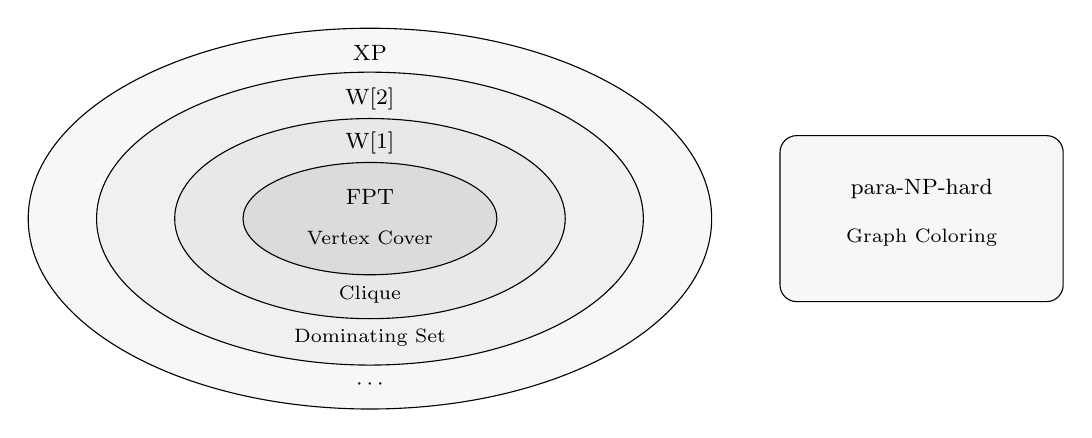
\begin{tikzpicture}[scale=0.62,every node/.style={font=\footnotesize},
    prob/.style={font=\scriptsize}]
  \draw[fill=black!3]  (0,0) ellipse (7.0 and 3.9);
  \draw[fill=black!6]  (0,0) ellipse (5.6 and 3.0);
  \draw[fill=black!9]  (0,0) ellipse (4.0 and 2.05);
  \draw[fill=black!14] (0,0) ellipse (2.6 and 1.15);
  \node[fill=black!3,inner sep=2pt] at (0,3.4)  {$\mathrm{XP}$};
  \node[fill=black!6,inner sep=2pt] at (0,2.45) {$\mathrm{W}[2]$};
  \node[fill=black!9,inner sep=2pt] at (0,1.55) {$\mathrm{W}[1]$};
  \node at (0,0.45) {$\mathrm{FPT}$};
  \node[prob] at (0,-0.4)  {\lang{Vertex Cover}};
  \node[prob] at (0,-1.55) {\lang{Clique}};
  \node[prob] at (0,-2.45) {\lang{Dominating Set}};
  \node at (0,-3.4)  {$\cdots$};
  % para-NP-hard sits outside XP altogether, unless P = NP
  \draw[fill=black!3,rounded corners=6pt] (8.4,-1.7) rectangle (14.2,1.7);
  \node at (11.3,0.6)  {para-\textrm{NP}-hard};
  \node[prob] at (11.3,-0.4) {\lang{Graph Coloring}};
\end{tikzpicture}
\caption{The parameterized classes and where the examples of this chapter sit.
The picture is drawn as if every inclusion were strict and $\mathrm{P} \neq
\mathrm{NP}$; only the inclusions themselves are theorems, and a para-\textrm{NP}-hard
problem lies outside $\mathrm{XP}$ exactly under that assumption.}
\label{fig:fpt-classes}
\end{figure}

The rest of the chapter is about the positive side: two techniques that put
problems into $\mathrm{FPT}$. There are others --- bounded treewidth
(\cref{ch:treewidth}) is one of them, and iterative compression another --- but
branching and kernelisation are the two that come first.

%==============================================================================
\section{Branching}
\label{sec:fpt-branching}
%==============================================================================

The idea is the one from \cref{ch:exact-i}, run with a different budget. Find a
small set of choices, one of which must be right; recurse on each; and arrange
that every recursive call decreases the parameter. The recursion then has depth
at most $k$, so if the branching factor is $b$ the search tree has at most $b^k$
leaves, and if the work per node is polynomial the algorithm is $\mathrm{FPT}$.

Four examples follow, in increasing order of how much thought the branching rule
takes.

\subsection{Vertex cover}

\begin{probdef}{Vertex Cover}
  \instance A graph $G = (V,E)$ and an integer $k$.
  \parameter $k$.
  \question Is there a set $C \subseteq V$ with $|C| \le k$ such that every edge
  has at least one endpoint in $C$?
\end{probdef}

The branching rule is as simple as a branching rule ever gets: pick any edge.
One of its two endpoints must be in the cover, since otherwise the edge is
uncovered.

\begin{algorithm}[ht]
\caption{Branching for \lang{Vertex Cover}}
\label{alg:fpt-vc}
\begin{algorithmic}[1]
  \Function{VC}{$G = (V,E)$, $k$}
    \If{$E = \emptyset$} \Return \textsc{true} \EndIf
    \If{$k = 0$} \Return \textsc{false} \EndIf
    \State select any edge $\{v,w\} \in E$
    \State \Return \Call{VC}{$G[V \setminus \{v\}]$, $k-1$} \textbf{ or }
                   \Call{VC}{$G[V \setminus \{w\}]$, $k-1$}
  \EndFunction
\end{algorithmic}
\end{algorithm}

\begin{figure}[ht]
\centering
\figplaceholder{5.5cm}{A small graph with a chosen edge $vw$ highlighted, and
below it the two children of the search tree: the graph with $v$ deleted and the
graph with $w$ deleted, each labelled with the decreased budget.}
\caption{One branching step for \lang{Vertex Cover}. Both children are smaller
instances with a smaller budget, and at least one of them is a yes-instance
whenever the parent is.}
\label{fig:fpt-vc-branch}
\end{figure}

\begin{theorem}\label{thm:fpt-vc}
\Cref{alg:fpt-vc} decides \lang{Vertex Cover} in $\bigoh{2^k(n+m)}$ time. Hence
\lang{Vertex Cover} is in $\mathrm{FPT}$.
\end{theorem}

\begin{proof}
\emph{Correctness.} If $E = \emptyset$ the empty set is a cover and $k \ge 0$
suffices. If $k = 0$ and edges remain, no cover of size $0$ exists. Otherwise
any cover must contain $v$ or $w$; if it contains $v$ then the rest of it is a
cover of $G - v$ of size at most $k-1$, and symmetrically for $w$. Conversely a
cover of $G - v$ of size $k-1$ becomes a cover of $G$ of size $k$ by adding $v$.
So the recursive calls return \textsc{true} for at least one child exactly when
the parent is a yes-instance.

\emph{Running time.} Each call decreases $k$ by one, so the search tree has
depth at most $k$ and at most $2^{k+1}$ nodes. Each node does $\bigoh{n+m}$ work
to find an edge and build the two subgraphs.
\end{proof}

\begin{remark}[The history of the constant]\label{rem:fpt-vc-history}
\lang{Vertex Cover} is the fruit fly of parameterized complexity, and the base
of its exponent has been pushed down for thirty years. The first
$\mathrm{FPT}$ algorithm, $\bigoh{f(k)n^3}$, came out of the graph minors
theorem and had an $f$ nobody could write down; \citet{BussGoldsmith1993} gave
$\bigoh{kn + 2^kk^{2k+2}}$ by the kernel of \cref{sec:fpt-vc-kernel};
$\bigoh{2^k(n+m)}$ is \cref{alg:fpt-vc}; and a long series of refinements by
increasingly careful case analysis reached $\bigoh{kn + 1.2738^k}$
\citep{ChenKanjXia2010}. The improvements are all in the branching rule: pick
the edge cleverly, and handle low-degree vertices separately.
\end{remark}

\subsection{Cluster editing}

The second example has a branching rule that needs a lemma. The problem comes
from biology: a similarity measurement is available for every pair of species,
and the species are to be partitioned into families --- but the measurements
contain errors, and we want to know how few.

\begin{probdef}{Cluster Editing}
  \instance An undirected graph $G = (V,E)$ and an integer $k$.
  \parameter $k$.
  \question Can at most $k$ modifications --- each the addition or the deletion
  of a single edge --- turn $G$ into a graph in which every connected component
  is a clique?
\end{probdef}

A graph all of whose components are cliques is called a \emph{cluster graph}.
The branching rule has to find, in a graph that is not one, a small set of
modifications one of which must be made. The following lemma supplies it.

\begin{lemma}\label{lem:cluster-p3}
$G$ is a cluster graph if and only if it contains no induced path on three
vertices. In particular, if some component of $G$ is not a clique, then there
are vertices $v,w,x$ with $\{v,w\} \in E$, $\{v,x\} \in E$ and
$\{w,x\} \notin E$.
\end{lemma}

\begin{proof}
An induced path $w - v - x$ has $w$ and $x$ in the same component and
non-adjacent, so no component containing one is a clique.

Conversely, suppose some component is not a clique. Then it contains two
non-adjacent vertices; among all such pairs in that component pick one, $w$ and
$x$, at minimum distance. That distance is at least $2$ because they are
non-adjacent, and it is at most $2$: if a shortest path $w, v, \ldots, x$ had
length more than $2$ then $v$ and $x$ would be a closer non-adjacent pair. So
the path is $w, v, x$ with $\{w,x\} \notin E$.
\end{proof}

\begin{algorithm}[ht]
\caption{Branching for \lang{Cluster Editing}}
\label{alg:fpt-cluster}
\begin{algorithmic}[1]
  \Function{CE}{$G$, $k$}
    \If{every component of $G$ is a clique} \Return \textsc{true} \EndIf
    \If{$k = 0$} \Return \textsc{false} \EndIf
    \State find $v,w,x$ with $\{v,w\},\{v,x\} \in E$ and $\{w,x\} \notin E$
           \Comment{\cref{lem:cluster-p3}}
    \State \Return \Call{CE}{$G - \{v,w\}$, $k-1$} \textbf{ or }
                   \Call{CE}{$G - \{v,x\}$, $k-1$} \textbf{ or }
                   \Call{CE}{$G + \{w,x\}$, $k-1$}
  \EndFunction
\end{algorithmic}
\end{algorithm}

\begin{theorem}\label{thm:fpt-cluster}
\Cref{alg:fpt-cluster} decides \lang{Cluster Editing} in
$\bigoh{3^k \cdot \poly(n)}$ time.
\end{theorem}

\begin{proof}
Consider a solution, that is a set of at most $k$ modifications producing a
cluster graph, and the three vertices $v,w,x$ that the algorithm found. In the
resulting graph, $w-v-x$ cannot remain an induced path, so the solution must
contain at least one of: the deletion of $\{v,w\}$, the deletion of $\{v,x\}$,
or the addition of $\{w,x\}$. Each branch performs one such modification and
decreases the budget, so one of the three branches leads to a solution using the
remaining $k-1$ modifications. The converse is immediate. The search tree has
depth $k$ and branching factor $3$.
\end{proof}

\begin{figure}[ht]
\centering
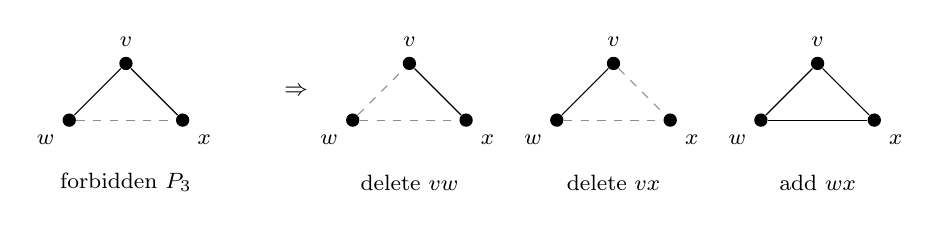
\begin{tikzpicture}[scale=0.72,
    vtx/.style={circle,fill=black,inner sep=1.7pt},
    miss/.style={black!45,dashed},
    every node/.style={font=\footnotesize}]
  % the forbidden induced path w - v - x
  \begin{scope}
    \node[vtx,label=above:$v$]      (v) at (0,1) {};
    \node[vtx,label=below left:$w$] (w) at (-1,0) {};
    \node[vtx,label=below right:$x$](x) at (1,0) {};
    \draw (w)--(v)--(x);
    \draw[miss] (w)--(x);
    \node at (0,-1.1) {forbidden $P_3$};
  \end{scope}
  % the three ways to destroy it
  \foreach \s/\dx/\cpt in {1/5/{delete $vw$}, 2/8.6/{delete $vx$},
      3/12.2/{add $wx$}}{
    \begin{scope}[xshift=\dx cm]
      \node[vtx,label=above:$v$]      (v\s) at (0,1) {};
      \node[vtx,label=below left:$w$] (w\s) at (-1,0) {};
      \node[vtx,label=below right:$x$](x\s) at (1,0) {};
      \node at (0,-1.1) {\cpt};
    \end{scope}
  }
  \draw[miss] (w1)--(v1); \draw (v1)--(x1); \draw[miss] (w1)--(x1);
  \draw (w2)--(v2); \draw[miss] (v2)--(x2); \draw[miss] (w2)--(x2);
  \draw (w3)--(v3)--(x3); \draw (w3)--(x3);
  \node at (3.0,0.5) {$\Rightarrow$};
\end{tikzpicture}
\caption{The branching rule for \lang{Cluster Editing}. The induced path on
three vertices must be destroyed, and there are only three ways to do it.}
\label{fig:fpt-cluster}
\end{figure}

\subsection{Independent set on planar graphs}

The third example shows the parameter interacting with structure: the same
problem that is $\mathrm{W}[1]$-complete on general graphs is $\mathrm{FPT}$ on
planar ones, and for an entirely elementary reason.

\begin{probdef}{Planar Independent Set}
  \instance A planar graph $G = (V,E)$ and an integer $k$.
  \parameter $k$.
  \question Does $G$ have an independent set of size at least $k$?
\end{probdef}

The branching rule uses the sparsity of planar graphs. By
\cref{ch:planar}, a planar graph has average degree less than $6$, so some
vertex $v$ has degree at most $5$.

\begin{lemma}\label{lem:planar-is-branch}
Let $v$ be any vertex and let $I$ be a maximum independent set. Then $I$
contains $v$ or one of its neighbours.
\end{lemma}

\begin{proof}
If $I$ contains no neighbour of $v$, then $I \cup \{v\}$ is independent, so by
maximality $v \in I$.
\end{proof}

So take a vertex $v$ of minimum degree, with neighbours $w_1, \ldots, w_r$ and
$r \le 5$, and branch on which of the $r+1 \le 6$ vertices
$v, w_1, \ldots, w_r$ is taken into the solution. Taking a vertex $x$ means
deleting $x$ together with all of its neighbours and decreasing $k$ by one.

\begin{theorem}\label{thm:fpt-planar-is}
\lang{Planar Independent Set} is solvable in $\bigoh{6^k n}$ time.
\end{theorem}

\begin{proof}
Correctness is \cref{lem:planar-is-branch} applied to the minimum-degree
vertex, together with the observation that deleting a chosen vertex and its
neighbours leaves exactly the instances in which the rest of the solution must
live. Deleting vertices keeps the graph planar, so the rule applies again at
every node. There are at most $6$ children per node and the depth is $k$.
\end{proof}

\begin{intuition}
There is a cheaper argument that gets a worse constant, and it is worth knowing
because it is the shape of many parameterized arguments. By the four colour
theorem a planar graph on $n$ vertices has an independent set of size at least
$n/4$. So if $k \le n/4$ the answer is \textsc{yes} without any computation, and
otherwise $n < 4k$ and the brute-force $\bigoh{2^n n}$ algorithm runs in
$\bigoh{2^{4k}k} = \bigoh{16^k k}$ time. Either the parameter is large enough
that the answer is forced, or the instance is small --- the same dichotomy that
\cref{sec:tw-minors} used with grid minors.
\end{intuition}

\subsection{Closest string}

The last example has a branching rule that is not about graphs at all, and where
the bound on the branching factor is the whole content.

\begin{probdef}{Closest String}
  \instance Strings $s_1, \ldots, s_k$, each of length $L$, and an integer $d$.
  \parameter $d$.
  \question Is there a string $s$ of length $L$ with Hamming distance at most
  $d$ to each of $s_1, \ldots, s_k$?
\end{probdef}

This is a consensus problem from molecular biology: the $s_j$ are observed
sequences and $s$ is the common ancestor they are all close to. Note that the
parameter is $d$, not the number of strings.

The algorithm searches for the solution by improving a candidate. A subproblem
is a pair $(s, r)$: the candidate $s$, and a budget $r$ of positions we are
still allowed to change in it. We start from $(s_1, d)$ and ask for a solution
of the original problem within Hamming distance $r$ of $s$.

\begin{algorithm}[ht]
\caption{Branching for \lang{Closest String}}
\label{alg:fpt-closest-string}
\begin{algorithmic}[1]
  \Function{CS}{$s$, $r$}
    \If{$d(s,s_j) \le d$ for every $j$} \Return $s$ \EndIf
    \State pick $j$ with $d(s,s_j) > d$
    \If{$d(s,s_j) > d + r$} \Return \textsc{false} \EndIf
    \For{each of the $d(s,s_j)$ positions $i$ where $s$ and $s_j$ differ}
      \State let $s'$ be $s$ with position $i$ set to $s_j(i)$
      \If{\Call{CS}{$s'$, $r-1$} succeeds} \Return its answer \EndIf
    \EndFor
    \State \Return \textsc{false}
  \EndFunction
\end{algorithmic}
\end{algorithm}

\begin{theorem}[\citet{GrammNiedermeierRossmanith2003}]\label{thm:fpt-closest-string}
\Cref{alg:fpt-closest-string}, called as $\textsc{CS}(s_1, d)$, decides
\lang{Closest String} in $\bigoh{(2d)^{d+1} \cdot kdL}$ time. Hence
\lang{Closest String} is in $\mathrm{FPT}$ parameterized by $d$.
\end{theorem}

\begin{proof}
\emph{The rejection test.} Suppose a solution $s^{*}$ within distance $r$ of $s$
exists. Then $d(s,s_j) \le d(s,s^{*}) + d(s^{*},s_j) \le r + d$, so the test on
line~4 rejects only hopeless subproblems.

\emph{The branching rule.} Let $P$ be the set of positions where $s$ and $s_j$
differ, so $|P| = d(s,s_j) > d$. Since $d(s^{*},s_j) \le d$, the solution
$s^{*}$ agrees with $s_j$ on at least $|P| - d \ge 1$ positions of $P$. Pick
such a position $i$: there $s^{*}(i) = s_j(i) \ne s(i)$, so setting position $i$
of $s$ to $s_j(i)$ makes $s$ agree with $s^{*}$ in one more place, and a
solution within distance $r-1$ of the new candidate still exists. The algorithm
tries every $i \in P$, so it tries this one.

\emph{Running time.} Every recursive call decreases $r$, which starts at $d$, so
the depth is at most $d$. At a node that branches, $|P| = d(s,s_j) \le d+r \le
2d$ by the rejection test, so the branching factor is at most $2d$ and the tree
has at most $(2d)^{d+1}$ nodes. Each node compares the candidate with all $k$
strings, at $\bigoh{kL}$ per comparison round, and the constant absorbs the
rest.
\end{proof}

\begin{example}\label{ex:closest-string}
Take $s_1 = 02231$, $s_2 = 01210$, $s_3 = 20221$ and $d = 2$. The first
subproblem is $(02231, 2)$. The candidate is at distance $0$, $3$ and $2$ from
the three strings, so $s_2$ witnesses failure; the two strings differ in
positions $2$, $4$ and $5$, and the call branches into
\[ (01231,\,1), \qquad (02211,\,1), \qquad (02230,\,1), \]
each obtained by copying one of those positions from $s_2$.

Take the first. Its distances are $1$, $2$ and $3$, so now $s_3$ witnesses
failure, and $3 \le d + r = 3$, so the rejection test lets it through. It
differs from $s_3$ in positions $1$, $2$ and $4$, giving
\[ (21231,\,0), \qquad (00231,\,0), \qquad (01221,\,0). \]
The first two are rejected at once: both are at distance $3$ from $s_2$, and
$3 > d + r = 2$. The third is at distance $2$ from all three strings, so
\textsc{CS} returns it on line~2, and $01221$ is the answer.
\end{example}

\subsection{The recipe}
\label{sec:fpt-branching-recipe}

All four algorithms are the same argument. To show a problem is in
$\mathrm{FPT}$ by branching, find a rule that
\begin{enumerate}[leftmargin=*,nosep]
  \item identifies a set of choices, at least one of which any solution must
        make;
  \item has a number of choices bounded by a function of the parameter --- a
        constant is best, but $2d$ was good enough above;
  \item decreases the parameter in every branch;
  \item costs polynomial time per node.
\end{enumerate}
The creative work is in~(1) and~(2), and the two go together: a rule that offers
too many choices is useless even if it is correct, which is why
\cref{lem:cluster-p3} and the bound $|P| \le 2d$ are the substance of their
respective proofs.

%==============================================================================
\section{Kernelisation}
\label{sec:fpt-kernelisation}
%==============================================================================

Every practitioner preprocesses: before running anything expensive, throw away
the parts of the instance that obviously cannot matter. Kernelisation is what
happens when that habit is given a guarantee. If the preprocessing is
polynomial and provably shrinks every instance to a size depending on $k$ alone,
then it is not a heuristic any more --- it is half of an algorithm.

\begin{definition}[Kernel]\label{def:kernel}
Let $P$ be a parameterized problem. A \emph{kernelisation} of $P$ is an
algorithm $A$ that maps an instance $(I,k)$ of $P$ to an instance
$A(I,k) = (I',k')$ of $P$ such that
\begin{enumerate}[label=(\roman*),leftmargin=*,nosep]
  \item $(I,k) \in P$ if and only if $(I',k') \in P$;
  \item $k' \le f(k)$ and $|I'| \le g(k)$, for computable functions $f$ and $g$;
  \item $A$ runs in time polynomial in $|I|$ and $k$.
\end{enumerate}
The reduced instance $(I',k')$ is the \emph{kernel}, and $g$ is its size. The
kernel is \emph{polynomial} if $g$ is a polynomial.
\end{definition}

Having a kernel is already an algorithm: reduce, then solve the kernel by brute
force, for a total of $p(n) + g'(f(k))$ time. The converse is also true, and
the proof is a trick worth seeing.

\begin{theorem}\label{thm:kernel-iff-fpt}
A decidable parameterized problem is in $\mathrm{FPT}$ if and only if it has a
kernel.
\end{theorem}

\begin{proof}
($\Leftarrow$) Given a kernelisation, compute the kernel in polynomial time and
then decide it by any algorithm at all --- the problem is decidable and the
kernel has size at most $g(k)$, so this costs a function of $k$ only. The total
is $\poly(n) + h(g(k))$, which is of the shape required by \cref{def:fpt}.

($\Rightarrow$) Suppose there is an algorithm running in time $f(k)\cdot n^{c}$.
Run it for $n^{c+1}$ steps. If it finishes, we know the answer, and we output a
constant-size yes-instance or no-instance accordingly --- a kernel of size
$\bigoh{1}$. If it does not finish, then $f(k)\cdot n^{c} > n^{c+1}$, hence
$n < f(k)$, and we output the input unchanged: it is already an instance of size
less than $f(k)$. Either way the output is a kernel, computed in $n^{c+1}$
steps.
\end{proof}

\begin{intuition}
\Cref{thm:kernel-iff-fpt} is one of those equivalences that is simultaneously
useful and disappointing. Useful, because it says kernelisation is not a
special trick but a complete characterisation of tractability. Disappointing,
because the kernel it produces in the forward direction has size $f(k)$, where
$f$ is whatever the algorithm's running time was --- possibly a tower of
exponentials. The interesting question is therefore never \emph{whether} a
kernel exists but how small it can be made, and specifically whether it can be
made polynomial. For some $\mathrm{FPT}$ problems the answer is provably no.
\end{intuition}

%==============================================================================
\section{A kernel for convex string recoloring}
\label{sec:fpt-convex-kernel}
%==============================================================================

The first worked kernel is on strings rather than graphs, which makes the
counting easy to see. It comes from phylogenetics: a character has been observed
along a sequence, each observation should form one contiguous stretch, and the
data does not quite do that.

\begin{probdef}{Convex String Recoloring}
  \instance A string $s$ over an alphabet of colours, and an integer $k$.
  \parameter $k$.
  \question Can at most $k$ characters of $s$ be changed so that $s$ becomes
  \emph{convex}, that is, so that for every colour the positions carrying it are
  consecutive?
\end{probdef}

For example \texttt{aaacccbxxxffff} is convex and \texttt{abba} is not. Three
pieces of vocabulary carry the argument. A \emph{block} is a maximal run of
consecutive equal characters, so \texttt{aabbacc} has four blocks. A colour is
\emph{good} if all its occurrences form a single block and \emph{bad}
otherwise; in \texttt{abba} the colour \texttt{a} is bad and \texttt{b} is good.
A string is convex exactly when every colour is good.

\begin{theorem}[\citet{MoranSnir2005}]\label{thm:convex-kernel}
\lang{Convex String Recoloring} has a kernel with $\bigoh{k^2}$ characters.
\end{theorem}

\begin{proof}
Three reduction rules, applied in order.

\emph{Rule 1: bound the number of bad blocks.} If $s$ has more than $4k$ blocks
of bad colours, return a trivial no-instance. This is correct because changing
one character alters only the block it lies in and its two neighbours, and can
turn at most one colour from bad to good; a case check shows the number of
blocks of bad colours drops by at most $4$. The string \texttt{abab} is the
tight case: it has four blocks and both of its colours are bad, so all four
blocks are blocks of bad colours, and changing the third character to
\texttt{b} gives \texttt{abbb}, in which both colours are good and no such block
is left. So $k$ changes cannot remove more
than $4k$ of them, and a convex string has none.

\emph{Rule 2: merge adjacent good blocks.} If two consecutive blocks both carry
good colours, recolour the second block with the colour of the first. This
neither helps nor hurts: a good colour is only ever recoloured in order to join
two blocks of a bad colour on either side of it, and doing that costs the same
before and after the merge. For example \texttt{abbbbcca} becomes
\texttt{abbbbbba}, and the instance \texttt{aaaaabbccaaaaa} with $k = 4$ becomes
\texttt{aaaaabbbbaaaaa} with $k = 4$.

\emph{Rule 3: bound the length of a block.} If a block has more than $k+1$
characters, delete all but $k+1$ of them. A block of that size cannot be
recoloured away with a budget of $k$, so the surviving copies play exactly the
same role as the originals. For example \texttt{aaaaabbbbbaa} with $k = 2$
becomes \texttt{aaabbbaa} with $k = 2$.

\emph{Counting.} Suppose all three rules have been applied. There are at most
$4k$ blocks of bad colours, by Rule~1. Between two consecutive bad blocks there
is now at most one good block, by Rule~2, and there is at most one more at each
end, so there are at most $4k+1$ blocks of good colours. Every block has at most
$k+1$ characters, by Rule~3. Hence
\[ |s| \;\le\; (4k + 4k + 1)(k+1) \;=\; (8k+1)(k+1) \;=\; \bigoh{k^2}. \]
Each rule is a linear scan and each application either shortens the string or
decreases the block count, so the whole reduction is polynomial.
\end{proof}

%==============================================================================
\section{A kernel for vertex cover}
\label{sec:fpt-vc-kernel}
%==============================================================================

The second kernel is the classical one, and it rests on three observations that
anyone would make after looking at a graph for a minute.

\begin{observation}\label{obs:fpt-vc-kernel}
Let $G$ be a graph and $k$ an integer.
\begin{enumerate}[label=(\roman*),leftmargin=*]
  \item An isolated vertex is in no minimal vertex cover and may be deleted.
  \item If $v$ has degree at least $k+1$, then $v$ belongs to every vertex cover
        of size at most $k$. Indeed, if $v$ is left out then all of its more
        than $k$ neighbours must be in the cover.
  \item If every vertex has degree at most $k$ and the graph has more than $k^2$
        edges, there is no vertex cover of size $k$: $k$ vertices of degree at
        most $k$ cover at most $k^2$ edges.
\end{enumerate}
\end{observation}

\begin{algorithm}[ht]
\caption{Kernelisation for \lang{Vertex Cover} }
\label{alg:fpt-vc-kernel}
\begin{algorithmic}[1]
  \State $H \gets G$, \quad $S \gets \emptyset$
  \While{$H$ has a vertex $v$ of degree at least $k+1$}
    \State remove $v$ and its incident edges from $H$
    \State $k \gets k-1$, \quad $S \gets S \cup \{v\}$
  \EndWhile
  \If{$k < 0$} \Return \textsc{false} \EndIf
  \If{$H$ has more than $k^2$ edges} \Return \textsc{false} \EndIf
  \State remove the isolated vertices of $H$
  \State \Return the instance $(H,k)$
\end{algorithmic}
\end{algorithm}

\begin{theorem}\label{thm:fpt-vc-kernel}
\Cref{alg:fpt-vc-kernel} runs in $\bigoh{n+m}$ time and returns a kernel with at
most $k^2$ edges and $2k^2$ vertices. Together with \cref{alg:fpt-vc} it decides
\lang{Vertex Cover} in $\bigoh{kn + 2^kk^2}$ time.
\end{theorem}

\begin{proof}
Every vertex removed in the loop is forced into the cover by
\cref{obs:fpt-vc-kernel}(ii), so $(G,k)$ is a yes-instance if and only if
$(H,k')$ is, where $k'$ is the decreased budget and $S$ is added to any cover
found. When the loop ends every remaining vertex has degree at most $k'$, so
\cref{obs:fpt-vc-kernel}(iii) justifies the rejection, and after it $H$ has at
most $k'^2$ edges. A graph with no isolated vertices has at most twice as many
vertices as edges.

Running the branching algorithm on the kernel costs
$\bigoh{2^{k}(n_H + m_H)} = \bigoh{2^kk^2}$. Producing the kernel is a single
pass, and the $kn$ term absorbs it: there is no solution at all once
$m > kn$, so the input may be assumed to have $\bigoh{kn}$ edges.
\end{proof}

\begin{intuition}
Notice how the two techniques compose. Kernelisation shrinks the instance from
$n$ to a function of $k$, and branching then pays the exponential price on the
small instance instead of the big one. That is the standard shape of a
parameterized algorithm, and it is why the two are taught together: kernelise
first, so that the $2^k$ multiplies $k^2$ rather than $n+m$.

\Cref{ch:kernelization} improves this kernel from $\bigoh{k^2}$ edges to $2k$
\emph{vertices}, using linear programming, and takes up the question of which
problems have polynomial kernels at all.
\end{intuition}

%==============================================================================
\section{Notes and further reading}
\label{sec:fpt-i-further-reading}
%==============================================================================

This chapter follows Hans Bodlaender's lecture slides. The textbooks are
\citet{DowneyFellows2013}, who founded the subject,
\citet{Niedermeier2006}, which is the gentlest introduction, and
\citet{CyganEtAl2015}, which is the current standard reference; branching is its
Chapter~3 and kernelisation its Chapter~2.

The $\bigoh{k^2}$ kernel for \lang{Vertex Cover} is \citet{BussGoldsmith1993},
and the long chain of improvements to the branching constant ends for now at
\citet{ChenKanjXia2010}. \Cref{thm:fpt-closest-string} is
\citet{GrammNiedermeierRossmanith2003} and \cref{thm:convex-kernel} is
\citet{MoranSnir2005}. \lang{Cluster Editing} was shown
\textrm{NP}-complete by \citet{ShamirSharanTsur2002}; faster branching
algorithms than \cref{alg:fpt-cluster} are known, and its kernel is in
\cref{ch:kernelization}.

%==============================================================================
\section{Exercises}
\label{sec:ex-fpt-i}
%==============================================================================

\begin{exercise}
\lang{Max SAT} asks whether at least $k$ clauses of a CNF formula can be
satisfied, with $k$ as the parameter. Give a branching algorithm showing it is
in $\mathrm{FPT}$. Hint: a variable occurring only positively, or only
negatively, can be set without branching; branching on any other variable
satisfies at least one clause on each side, so what happens to $k$?
\end{exercise}

\begin{exercise}
Show that \lang{Vertex Cover} parameterized by $n - k$ --- can all but $k$
vertices be deleted so that the rest is a cover? --- is
$\mathrm{W}[1]$-hard. Hint: what is the complement of a vertex cover?
\end{exercise}

\begin{exercise}
In \cref{alg:fpt-vc}, replace ``select any edge'' by ``select an edge incident
to a vertex of maximum degree''. Show that if the maximum degree is at least
$3$, the branching vector improves, and estimate the resulting base of the
exponent.
\end{exercise}

\begin{exercise}
\Cref{lem:cluster-p3} produces one induced path on three vertices. Show that if
two such paths are vertex-disjoint, the branching can be done on both at once,
and say what that gives.
\end{exercise}

\begin{exercise}
Give an example showing that \cref{alg:fpt-cluster} may add an edge that a later
branch deletes again. Why does this not affect correctness, and how would you
avoid it in an implementation?
\end{exercise}

\begin{exercise}
Prove the claim used in \cref{thm:fpt-planar-is} that deleting vertices from a
planar graph leaves a planar graph, and explain why the same branching rule
gives $\bigoh{(\Delta+1)^k n}$ on any graph of maximum degree $\Delta$.
\end{exercise}

\begin{exercise}
In \cref{alg:fpt-closest-string}, show that the algorithm may safely skip any
position that was changed by an earlier call on the current root-to-node path,
and bound how much this saves.
\end{exercise}

\begin{exercise}
Show that \lang{Closest String} parameterized by the number $k$ of strings,
rather than by $d$, is not obviously in $\mathrm{FPT}$: where does the argument
of \cref{thm:fpt-closest-string} break?
\end{exercise}

\begin{exercise}
Rule~1 of \cref{thm:convex-kernel} uses the bound $4$. Work out the case
analysis, and show that any constant bound in place of $4$ still yields an
$\bigoh{k^2}$ kernel.
\end{exercise}

\begin{exercise}
\Cref{thm:kernel-iff-fpt} produces a kernel of size $f(k)$ from an
$f(k)n^c$-time algorithm. Apply the construction to \cref{alg:fpt-vc} and
compare the kernel it yields with the one of \cref{thm:fpt-vc-kernel}.
\end{exercise}
